\documentclass[journal=jacsat,manuscript=article]{achemso}
\usepackage[parfill]{parskip}
\usepackage[version=3]{mhchem} % Formula subscripts using \ce{}
\usepackage[section]{placeins}
\newcommand*\mycommand[1]{\texttt{\emph{#1}}}


\title{polypy - Something interesting needed here}
\author{Adam R. Symington}
\email{A.R.Symington@bath.ac.uk}
\affiliation{Department of Chemistry, University of Bath, Claverton Down, Bath BA2 7AY, UK}
\author{Stephen C. Parker}
\email{S.C.Parker@bath.ac.uk}
\affiliation{Department of Chemistry, University of Bath, Claverton Down, Bath BA2 7AY, UK}

\date{2019\\ March}

\begin{document}


%\textbf{Paper DOI:}  \\
%\textbf{Software Repository:} \\
%\textbf{Software Archive:}  \\

\section{Summary}
A large number of research questions in solid state chemistry can be addressed using molecular dynamics and Monte Carlo simulations. These simulations allow many material properties to be calculated for direct comparison with experiment.  These include, the diffusion coefficients of lithium ions in battery materials or oxygen atoms in SOFCs, segregation behaviour of defects at grain boundaries, the dynamics of water at material surfaces and as well as many others.

A molecular dynamics trajectory is a snapshot of the positions of each atom as a function time e.g. the trajectory of a single atom would show, sequentially, all of the postiions occupied by that atom throughout the simulaton. The positions of the atoms as a function of time allows the partcle densitites to be calculated and thus the charge densities e.g. Figure 1. The charge densities can be used to calculate the electric field across the unit cell, and also the electrostatic potential.   

\begin{figure}[!htb]
    \centering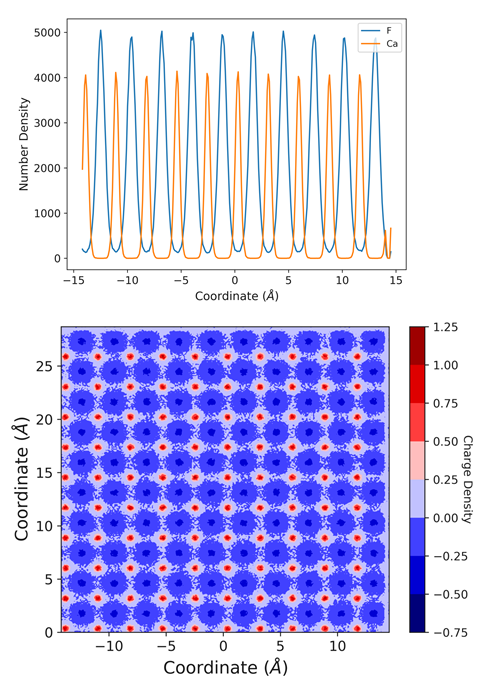
\includegraphics[width=4in]{../Figure_1.png}
    \caption{This figure illustrates an example one dimensional particle density plot (a), and two dimensional charge density plot (b).}
    \label{Figure 1}
  \end{figure}

The atomic trajectories as a function of time also allow diffusion coefficients to be calculated using a mean squared displacement. Using a dye molecule in water as an example, the motion of a dye molecule is not simple. As it moves it is jostled by collisions with other molecules, preventing it from moving in a straight path. If the path is examined in close detail, it will be seen to be a good approximation to a random walk. In mathmatics a random walk is a series of steps, each taken in a random direction. This was analysed by Albert Einstein in a study of Brownian motion and he showed that the mean square of the distance travelled by a particle following a random walk is proportional to the time elapsed. 

\begin{align}
\Big \langle r_{i}^{2} \big \rangle & = 6 D_t + C 
\end{align}

where 

\begin{align}
\Big \langle r_{i}^{2} \big \rangle = \frac{1}{3} \Big< | r_{i}(t) - r_{i}(0) |^2 \Big>.
\end{align}


where $\Big \langle r^2 \big \rangle$ is the mean squared distance, t is time, $D_t$ is the diffusion rate and C is a constant. If $\Big \langle r_{i}^{2} \big \rangle$ is plotted as a function of time, the gradient of the curve obtained is equal to 6 times the self-diffusion coefficient of particle i.

\section{polypy}

`polypy` is a Python module for analysing trajectories generated from molecular dynamics and Monte Carlo data specifically from the DL\_POLY and DL\_MONTE codes, athough the code is designed for the integration of other codes.
It contains two core modules for designed to perform density analysis and mean squared displacements.
These allow the calculation of one and two dimensional particle/charge densities, electric fields, electrostatic potentials and diffusion coefficients. A module allowing easy generation of publication plots from the calculated data is available, but the outputs are returned in a sensible form, allowing further manipulation and plotting.
`polypy` is aimed towards theoretical solid state physicist who have a basic familiarity with Python.
The repository contains examples of the core functionality as well as tutorials, implemented in Jupyter notebooks to explain the full theory.
Furthermore, a detailed description of theory is also available within the documentation.

\section{Acknowledgments}

ARS would like to thank Andrew R. McCluskey for his guidance through this project and Benjamin Morgan for his help with the Poisson Boltzmann calculation. This package was written during a PhD funded by AWE and EPSRC (EP/R010366/1). The input data for the development and testing of this project was generated using ARCHER UK National Supercomputing Service (http://www.archer.ac.uk) via our membership of the UK's HEC Ma-terials Chemistry Consortium funded by EPSRC (EP/L000202).
%\bibliography{paper}

\end{document}